\documentclass[titlepage,dvipdfmx]{jsarticle}
\usepackage{graphicx}
\usepackage{amsmath,amssymb}
\usepackage{fancyvrb}
\usepackage{cases}
\usepackage{here}
\usepackage{capt-of}
\usepackage{multirow}
%\usepackage{my-report}
%\usepackage{newtxtext,newtxmath}
\usepackage{fancyvrb}
\usepackage{listings}
\usepackage{comment}
\usepackage{pdfpages}
\usepackage{siunitx}
\usepackage{subcaption}
\lstset{
    basicstyle={\ttfamily},
    identifierstyle={\small},
    commentstyle={\small\itshape},
    keywordstyle={\small\bfseries},
    ndkeywordstyle={\small},
    stringstyle={\small\ttfamily},
    frame={tb},
    breaklines=true,
    columns=[l]{fullflexible},
    numbers=left,
    xrightmargin=0zw,
    xleftmargin=3zw,
    numberstyle={\scriptsize},
    stepnumber=1,
    numbersep=1zw,
    lineskip=-0.5ex,
    keepspaces=true,
    language=c++
}
\renewcommand{\lstlistingname}{ソースコード}
\makeatletter
\newcommand{\figcaption}[1]{\def\@captype{figure}\caption{#1}}
\newcommand{\tblcaption}[1]{\def\@captype{table}\caption{#1}}
\makeatother
\fvset{
  fontsize=\small,%  フォントサイズをsmallに
  frame=single,%     枠で囲う (lines でもよいかも)
  numbers=left,%     左に行番号を付ける
  tabsize=4,%        タブは半角4文字分に変換
  baselinestretch=0.8%  行送りを標準の0.8倍に詰める
}
\newcommand{\Figref}[1]{\figurename~\ref{#1}}
\newcommand{\Tblref}[1]{\tablename~\ref{#1}}

\title{\Huge{数値解析レポートNo.3}}
\author{\huge{43番 若月 耕紀}}
\date{}

\begin{document}
\maketitle
\newpage


\section{多項式以外の一般的な近似法の1つに指数近似\protect\linebreak
\centerline{$y = a_0 e^{a_1 x}$}\protect\linebreak
がある.\protect\linebreak
以下のデータを指数近似してグラフを示せ.\protect\linebreak
(x, y) = (1.5, 8.96), (2.0, 14.78), (2.5, 24.36), (3.0, 40.17)}

指数近似の両辺対数を取ると,$\ln y = \ln a_0 + a_1 x$となり,線形近似と同じになる.これを用いて指数近似を行う関数をソースコード1に示す.

\begin{lstlisting}[caption=exp\_app, label=src:exp]
#define A_NUM 2
#define DATA_NUM 4

void exp_app(double *x, double *y, double *a){
	double *b = allocVector(A_NUM), **A = allocMatrix(A_NUM, A_NUM);
	int i, j, k;

	//左辺
	for(j = 0; j < A_NUM; j++){
		for(k = 0; k < DATA_NUM; k++){
			b[j] += log(y[k]) * pow(x[k], j);
		}
	}

	//右辺
	for(j = 0; j < A_NUM; j++){
		for(i = j; i < A_NUM; i++){
			for(k = 0; k < DATA_NUM; k++){
				A[j][i] += pow(x[k], (j + i));
			}
		}
	}
	//対称行列
	A[j - 1][i - 2] = A[i - 2][j - 1];

	//ガウスの消去法
	gauss_elim(a, b, A);

	a[0] = exp(a[0]);
}
\end{lstlisting}

講義資料にある手順と同様に,左辺,右辺をそれぞれ求め,その後にガウスの消去法で$a_0, a_1$を求める.また,$a_0$については$\ln a_0$として計算されているため,調整を行う.

この関数を使って与えられたデータを近似すると$a_0 \approx 2.00$,$a_1 \approx 1.00$が得られる.与えられたデータと$y = 2e^{x}$をプロットしたものをグラフ1に示す.

\begin{figure}[htbp]
  \begin{center}
    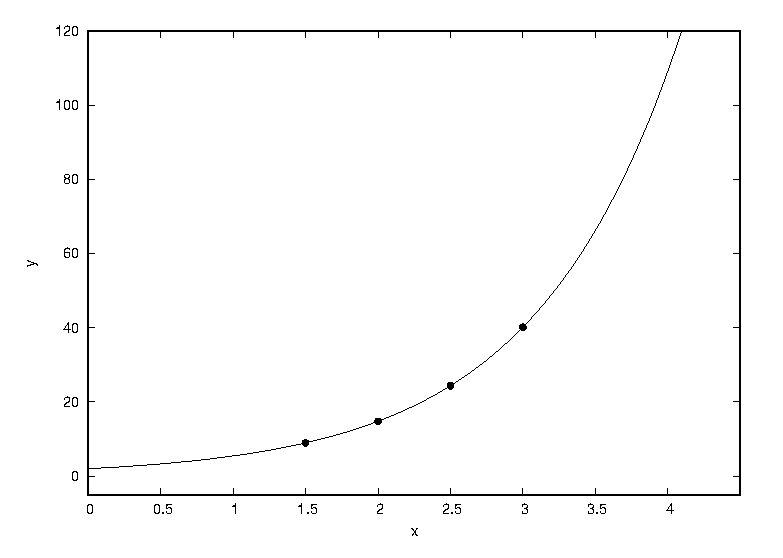
\includegraphics[width=13cm]{main.eps}
    \caption{指数近似}
    \label{q12}
  \end{center}
\end{figure}

図より,適切に近似できていることが分かる.

\section{(サービス問題)\protect\linebreak
これまでに行った相互評価について,\protect\linebreak
 $\bullet$良いと思うところ,参考になったところ\protect\linebreak
 $\bullet$改善すべきところ,改善案,バグ報告\protect\linebreak
 $\bullet$疑問,感想\protect\linebreak
をまとめて提出する.}

\subsubsection*{$\bullet$良いと思うところ,参考になったところ}
他人のコードを見ると,見やすいコードと見にくいコードの違いが明確になるため,自分でコードを書くときに,見やすいコードを意識しながら書くことができる.また,同じ目的のコードでも,処理が違うと異なった視点から考えることができるため,より深く内容を理解することができる.

これまでの相互評価では特にコメントの使い方が参考になった.コメントの書き方でコードの理解度がかなり変わってくるため,今後は適切なコメントを書くようにしたい.

\subsubsection*{$\bullet$改善すべきところ,改善案,バグ報告}
相互評価終了後に他人のコードを見ることができなくなるため,相互評価後も見られるようにした方が良いと思う.理由としては,相互評価は,他人のコードを見て学ぶことに意義があると考えているため,いつでも見られた方が,より学ぶことができるのではないかと考える.

\subsubsection*{$\bullet$疑問,感想}
全体的にみて,相互評価は自分のためになったと思う.自分のコードだけ見ていると変な癖がついてしまい,共同開発をするときに苦労することになる.そのため,早い段階から他人のコードを見る機会が作れる相互評価は良かったと思う.

\section{解析的に解ける非線形関数を,台形・シンプソン・ロンバーグの3手法により数値積分し,それぞれの\protect\linebreak
 (1)分割数と誤差\protect\linebreak
 (2)計算量(計算速度)\protect\linebreak
について調査し報告せよ.関数,積分区間,分割数は適切に設定すること.}
台形公式,シンプソン公式,ロンバーグ法の3手法により,定積分を行う関数をソースコード2に示す.

\begin{lstlisting}[caption=exp\_app, label=src:exp]
//台形公式  ( 分割数a0, 積分範囲[a1, a2] )
void trapezoid(double a0, double a1, double a2){
	double k, h, sum = 0;

	h = (a2 - a1) / a0;

	for(k = a1 + h; k < a2; k += h){
		sum += f(k);
	}

	printf("T = %f", (h / 2.0) * (f(a1) + f(a2) + (2.0 * sum)));
}

//シンプソン公式 ( 分割数a0, 積分範囲[a1, a2] )
void simpson(double a0, double a1, double a2){
	double k, h, sum1 = 0, sum2 = 0;

	h = (a2 - a1) / a0;

	for(k = a1 + h; k < a2; k += h){
		sum1 += f(k);
		k += h;
		if(k < a2) sum2 += f(k);
	}

	printf("S = %f", (h / 3.0) * (f(a1) + f(a2) + (4.0 * sum1) + (2.0 * sum2)));
}

//ロンバーグ法 ( 積分範囲[a1, a2] )
void romberg(double a1, double a2){
	int i, k, m;
	double h, sum, T[N + 1][N + 1];

	//2^0 = 1 分割の台形公式
	h = a2 - a1;
	T[0][0] = h * (f(a1) + f(a2)) / 2;
	
	for(k = 1; k <= N; k++) {
		h /= 2;

		for(i = 1, sum = 0; i <= pow(2, (k - 1)); i++){
			sum += f(a1 + (2 * i - 1) * h);
		}
		T[k][0] = T[k - 1][0] / 2.0 + h * sum;

		for(m = 1; m <= k; m++){
			T[k][m] = T[k][m - 1] + (T[k][m - 1] - T[k - 1][m - 1]) / (pow(4, m) - 1);
			//収束判定
			if(fabs(T[k][m] - T[k][m - 1]) < EPS) break;
		}

		//収束判定
		if(fabs(T[k][0] - T[k - 1][0]) < EPS) break;
	}

	printf("分割数:%d, 次数:%d\n", (int)pow(2, k), (int)pow(2, m));
	printf("R = %f", T[k - 1][m - 1]);
}
\end{lstlisting}

台形公式については,シグマの部分をfor文で先に計算を行い,最後に公式を出力させた.

シンプソン公式については,奇数番目と偶数番目を分けなければならないため,for文内でもk += hを計算している.

ロンバーグ法については,まず初期値を求める.その後,講義資料にある公式に従って二重のforループ処理を行った.

\subsection*{(1)分割数と誤差}
ソースコード2のプログラムを用いて,$y = \sin x\:(0 \leqq x \leqq \pi / 2)$と$y = e^x\:(0 \leqq x \leqq 2)$の定積分を求める.

誤差を推移を調べるために,理論値を求める.理論値は以下のようになる.
\begin{eqnarray}
&&\int_0^{\pi / 2}\sin x = 1 \nonumber\\
&&\int_0^2 e^x = e^2 - 1 \approx 6.389056099 \nonumber
\end{eqnarray}

各分割数についての理論値と計算結果との差をプロットしたものを図2, 3に示す.

グラフを見ると,どちらの式でも分割数の増加に伴い,誤差が減少していることがわかる.また,収束の速度は,ロンバーグ法,シンプソン公式,台形公式の順で速くなっていることがわかる.

台形公式とシンプソン公式については分割数が大きくなっても誤差が出ることがあるが,ロンバーグ法については,分割数が小さい段階から既に誤差が少なく,分割数が大きくなると完全に収束していることがわかる.

\begin{figure}[h]
\begin{minipage}{0.5\hsize}
	\centering
	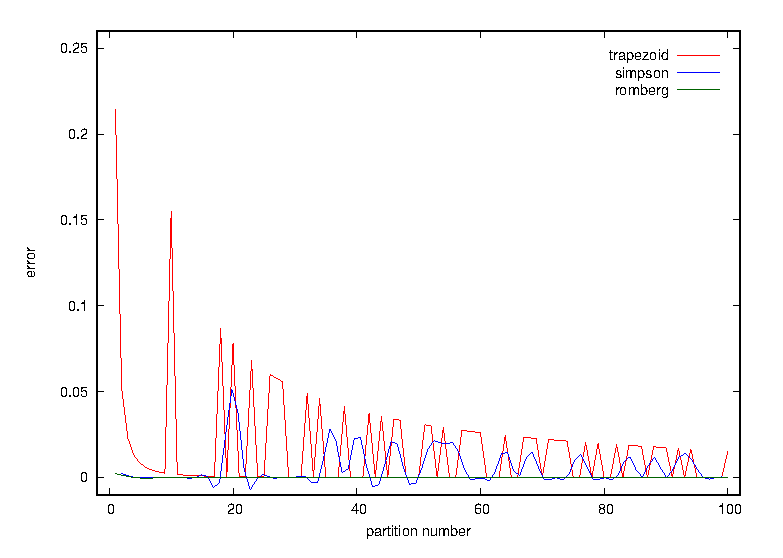
\includegraphics[width=8cm]{sin.eps}
	\caption{$y = \sin x$}
	\label{fig:4-1}
\end{minipage}
\begin{minipage}{0.5\hsize}
	\centering
	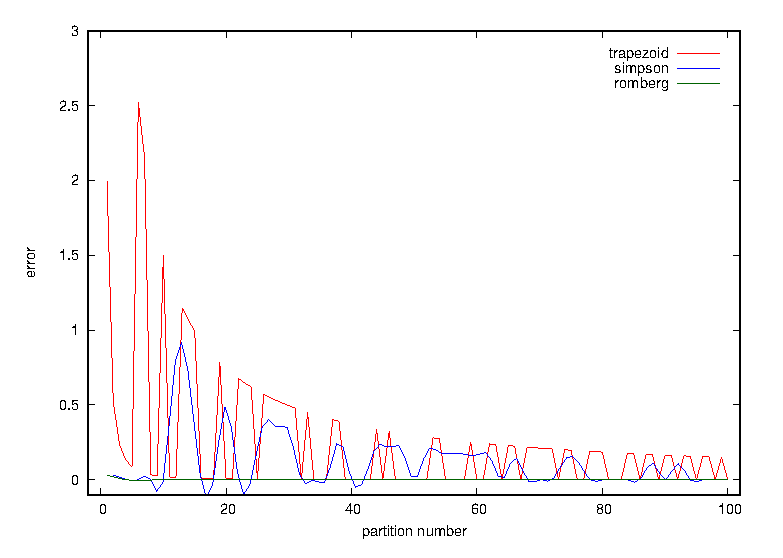
\includegraphics[width=8cm]{e.eps}
	\caption{$y = e^x$}
	\label{fig:4-2}
\end{minipage}
\label{fig:5}
\end{figure}

\subsection*{(2)計算量(計算速度)}
台形公式と,シンプソン公式は,データ数$N$回のループ処理を行っているため,計算量は$O(N)$となる.ロンバーグ法は,二重のループ処理を行っているため,計算量は$O(N^2)$となる.

計算量だけを見ると,台形公式やシンプソン公式の方が良いといえるが,ロンバーグ法は少ない分割数で正確な値を計算することができるため,分割数を多くしなければならないというような特別な理由がない限りはロンバーグ法で定積分を行う方が良いといえる.

\section{感想}
今回は,想定よりも難しかったと感じた.出力結果が少し違ったときにプログラムのどこが間違えているのかがなかなか見つけられず,かなり時間がかかった.また,今回のレポートは以前より早く取り組み始めることができた.しかし,予想よりも時間がかかってしまったため,今回の経験を活かして,今後は計画を立てながら進めようと思う.



\begin{thebibliography}{99}
\bibitem{text} 「計算量オーダーについて」
https://qiita.com/asksaito/items/59e0d48408f1eab081b5
\end{thebibliography}

\end{document}